\documentclass[uplatex, dvipdfmx]{jsarticle}


\usepackage{tcolorbox}
\usepackage{color}
\usepackage{listings, plistings}

%% ノート/latexメモ
%% http://pepper.is.sci.toho-u.ac.jp/pepper/index.php?%A5%CE%A1%BC%A5%C8%2Flatex%A5%E1%A5%E2

%% JavaScriptの設定
%% https://e8l.hatenablog.com/entry/2015/11/29/232800
\lstdefinelanguage{javascript}{
  morekeywords = [1]{ %keywords
    await, break, case, catch, class, const, continue, debugger, default, delete, 
    do, else, enum, export, extends, finally, for, function, function*, if, implements, import, in, 
    instanceof, interface, let, new, package, private, protected, public, return, static, super,
    switch, this, throw, try, typeof, var, void, while, with, yield, yield*
  },
  morekeywords = [2]{ %literal
    false, Infinity, NaN, null, true, undefined
  },
  morekeywords = [3] { %Classes
    Array, ArrayBuffer, Boolean, DataView, Date, Error, EvalError, Float32Array, Float64Array,
    Function, Generator, GeneratorFunction, Int16Array, Int32Array, Int8Array, InternalError,
    JSON, Map, Math, Number, Object, Promise, Proxy, RangeError, ReferenceError, Reflect,
    RegExp, Set, String, Symbol, SyntaxError, TypeError, URIError, Uint16Array, Uint32Array,
    Uint8Array, Uint8ClampedArray, WeakMap, WeakSet
  },
  morecomment = [l]{//},
  morecomment = [s]{/*}{*/},
  morestring = [b]{"},
  morestring = [b]{'},
  alsodigit = {-},
  sensitive = true
}

%% 修正時刻: Tue 2022/03/15 10:04:41


% Java
\lstset{% 
  frame=single,
  backgroundcolor={\color[gray]{.9}},
  stringstyle={\ttfamily \color[rgb]{0,0,1}},
  commentstyle={\itshape \color[cmyk]{1,0,1,0}},
  identifierstyle={\ttfamily}, 
  keywordstyle={\ttfamily \color[cmyk]{0,1,0,0}},
  basicstyle={\ttfamily},
  breaklines=true,
  xleftmargin=0zw,
  xrightmargin=0zw,
  framerule=.2pt,
  columns=[l]{fullflexible},
  numbers=left,
  stepnumber=1,
  numberstyle={\scriptsize},
  numbersep=1em,
  language={Java},
  lineskip=-0.5zw,
  morecomment={[s][{\color[cmyk]{1,0,0,0}}]{/**}{*/}},
  keepspaces=true,         % 空白の連続をそのままで
  showstringspaces=false,  % 空白字をOFF
}
%\usepackage[dvipdfmx]{graphicx}
\usepackage{url}
\usepackage[dvipdfmx]{hyperref}
\usepackage{amsmath, amssymb}
\usepackage{itembkbx}
\usepackage{eclbkbox}	% required for `\breakbox' (yatex added)
\usepackage{enumerate}
\usepackage[default]{cantarell}
\usepackage[T1]{fontenc}
\fboxrule=0.5pt
\parindent=1em
\definecolor{mygrey}{rgb}{0.97, 0.97, 0.97}

\makeatletter
\def\verbatim@font{\normalfont
\let\do\do@noligs
\verbatim@nolig@list}
\makeatother

\begin{document}

%\anaumeと入力すると穴埋め解答欄が作れるようにしてる。\anaumesmallで小さめの穴埋めになる。
\newcounter{mycounter} % カウンターを作る
\setcounter{mycounter}{0} % カウンターを初期化
\newcommand{\anaume}[1][]{\refstepcounter{mycounter}{#1}{\boxed{\phantom{aa}\textnormal{\themycounter}\phantom{aa}}}} %穴埋め問題の空欄作ってる。
\newcommand{\anaumesmall}[1][]{\refstepcounter{mycounter}{#1}{\boxed{\tiny{\phantom{a}\themycounter \phantom{a}}}}}%小さい版作ってる。色々改造できる。

%% 修正時刻: Tue 2022/03/15 10:04:411


\section{MAMPのインストール}

\subsection{MAMPのダウンロード}

\textsf{MAMP}で検索すると、このサイトに行くことができる。

\vspace{3mm}
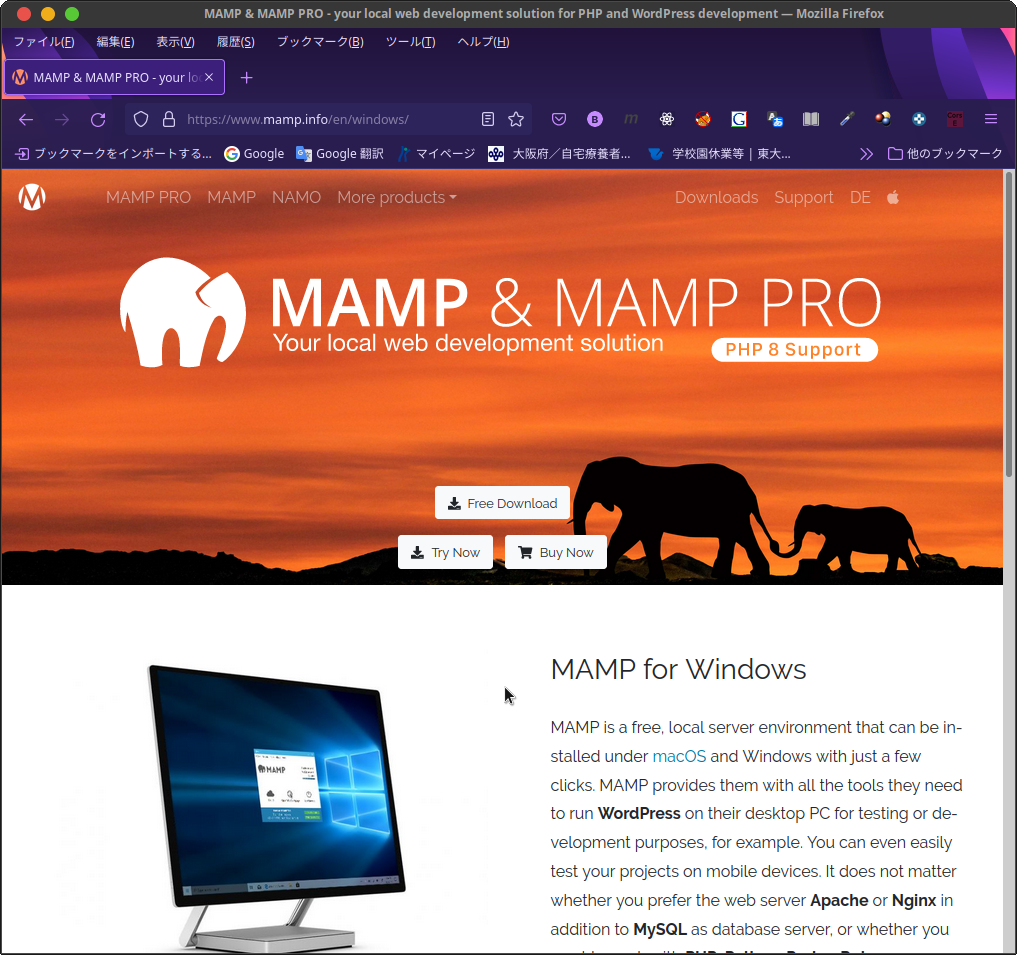
\includegraphics[width=10cm]{img/00-01-mamp-site.png}
\vspace{3mm}

\textsf{Free Download} をクリックする。以下の画面になる。

\vspace{3mm}
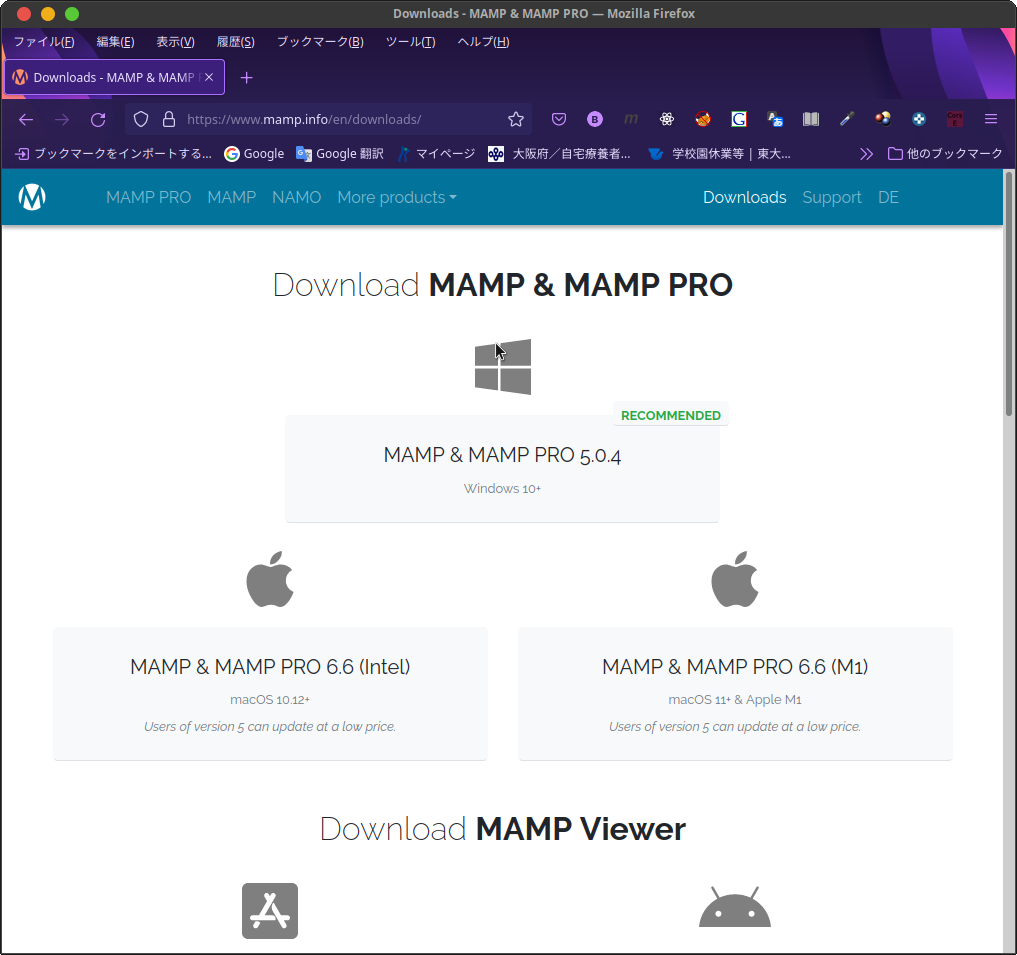
\includegraphics[width=10cm]{img/00-02-download.png}
\vspace{3mm}

Windowsの ``MAMP \& MAMP PRO 5.0.4''を選択する。

\vspace{3mm}
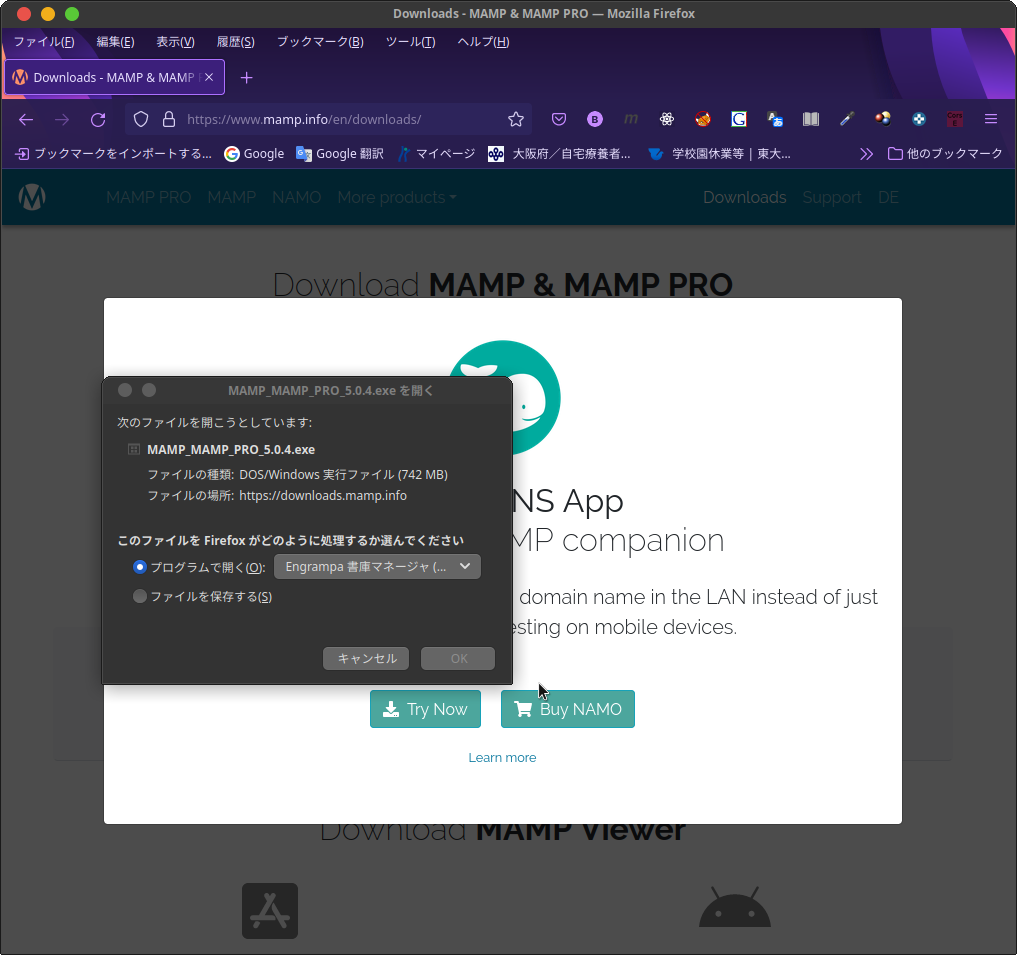
\includegraphics[width=10cm]{img/00-03-mamp-save.png}
\vspace{3mm}

MAMP companion の宣伝が表示されるが、何もせずにいると、
「MAMP\_MAMP\_PRO\_5.0.4.exe」の保存ができるようになる。

保存が終わったら、MAMP\_MAMP\_PRO\_5.0.4.exe をクリックすると、
インストールが始まる。

\vspace{3mm}
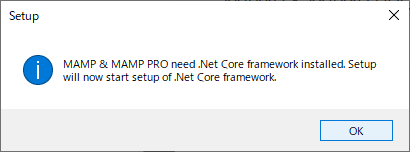
\includegraphics[width=10cm]{img/01-install.png}
\vspace{3mm}

``OK''をクリックする。

\vspace{3mm}
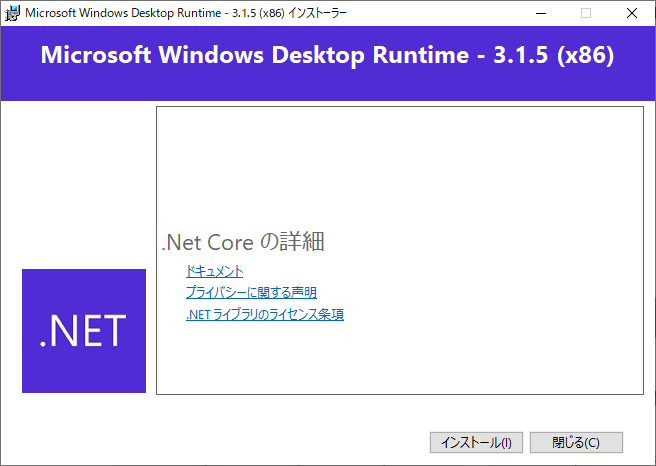
\includegraphics[width=10cm]{img/02-net-core.png}
\vspace{3mm}

``インストール''をクリックする。

\vspace{3mm}
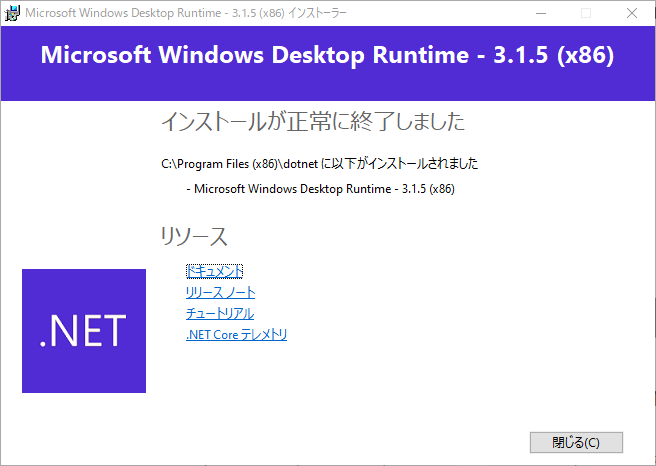
\includegraphics[width=10cm]{img/03-net-core-finish.png}
\vspace{3mm}

``閉じる''をクリックする。

\vspace{3mm}
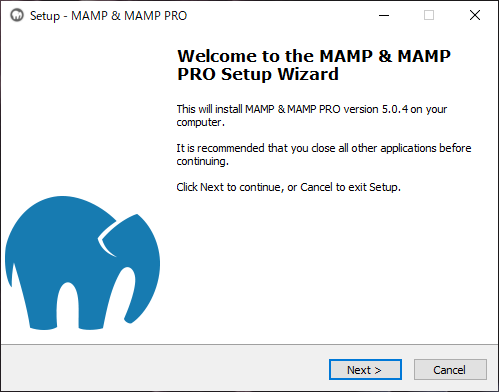
\includegraphics[width=10cm]{img/04-mamp-install.png}
\vspace{3mm}

``Next >''をクリック。

\vspace{3mm}
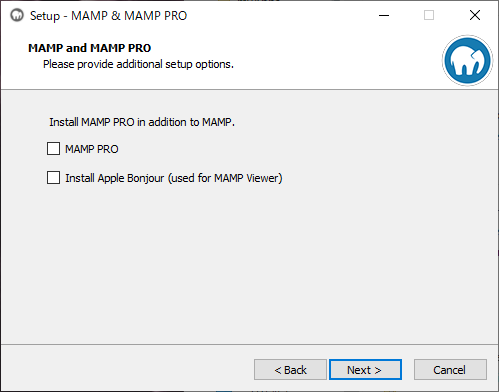
\includegraphics[width=10cm]{img/05-mamp-select.png}
\vspace{3mm}

どちらも選択しない。(MAMP PROは有料だし、MAMP Viewerは使わないし。)

\vspace{3mm}
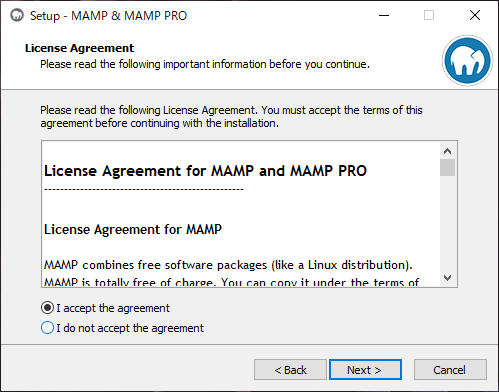
\includegraphics[width=10cm]{img/06-mamp-install.png}
\vspace{3mm}

ライセンスに同意する。(I accept the agreement)

``next >''をクリック。

\vspace{3mm}
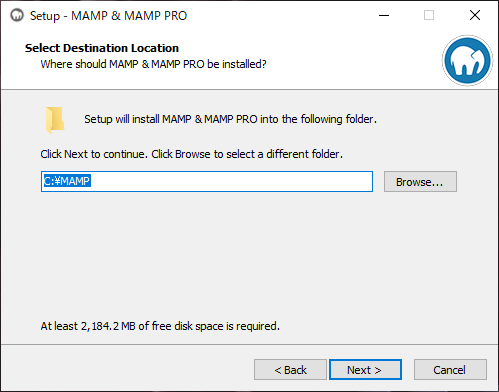
\includegraphics[width=10cm]{img/07-install-dir.png}
\vspace{3mm}

C:\yen MAMP にインストールされる。それでいい。

\vspace{3mm}
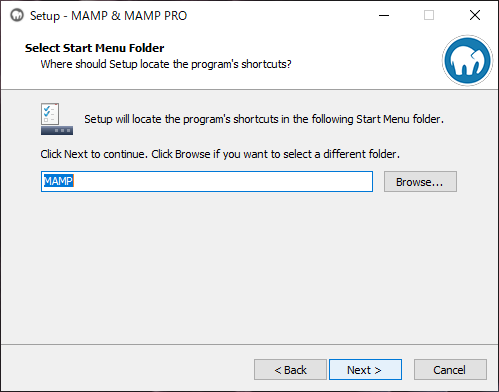
\includegraphics[width=10cm]{img/08-install-name.png}
\vspace{3mm}

スタートメニューに MAMP という項目ができる。それでいい。

\vspace{3mm}
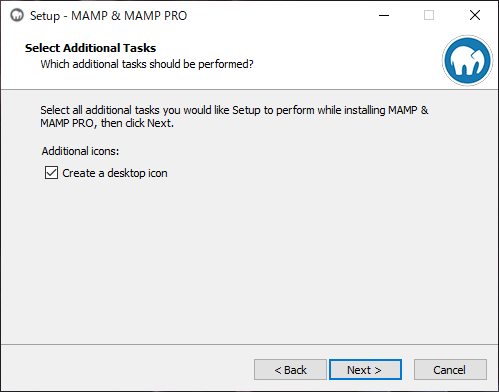
\includegraphics[width=10cm]{img/09-create-icon.png}
\vspace{3mm}

デスクトップにショートカットアイコンができる。それでいい。

\vspace{3mm}
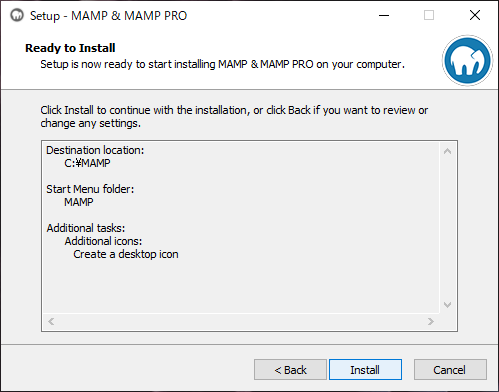
\includegraphics[width=10cm]{img/10-install-confirm.png}
\vspace{3mm}

これでインストールは完了。

MAMPを起動する。

\vspace{3mm}
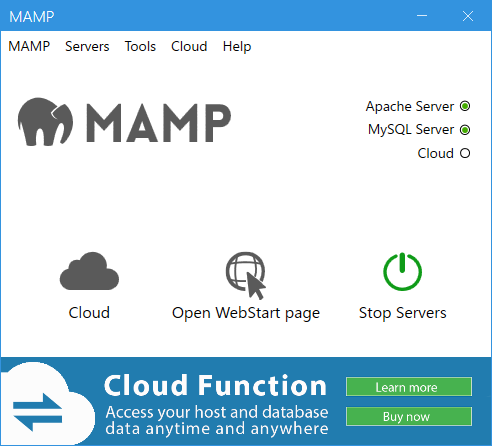
\includegraphics[width=10cm]{img/12-mamp.png}
\vspace{3mm}

起動と同時に Apache と MySQL が起動して、緑色のランプがつく。


確認画面。

\vspace{3mm}
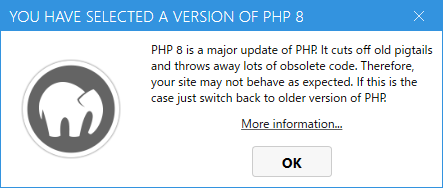
\includegraphics[width=10cm]{img/11-php-version.png}
\vspace{3mm}

「あなたは PHP8 を選択しました」\dots\dots みたいな \dots\dots。




\end{document}

%% 修正時刻: Sat May  2 15:10:04 2020


%% 修正時刻: Wed 2022/04/06 06:22:582
